\documentclass[border=2pt]{standalone}
\usepackage{pgfplots}
\pgfplotsset{compat=1.18}
\definecolor{forgeblue}{HTML}{2166AC}
\definecolor{forgeorange}{HTML}{B35806}
\definecolor{forgegreen}{HTML}{167D5B}
\begin{document}
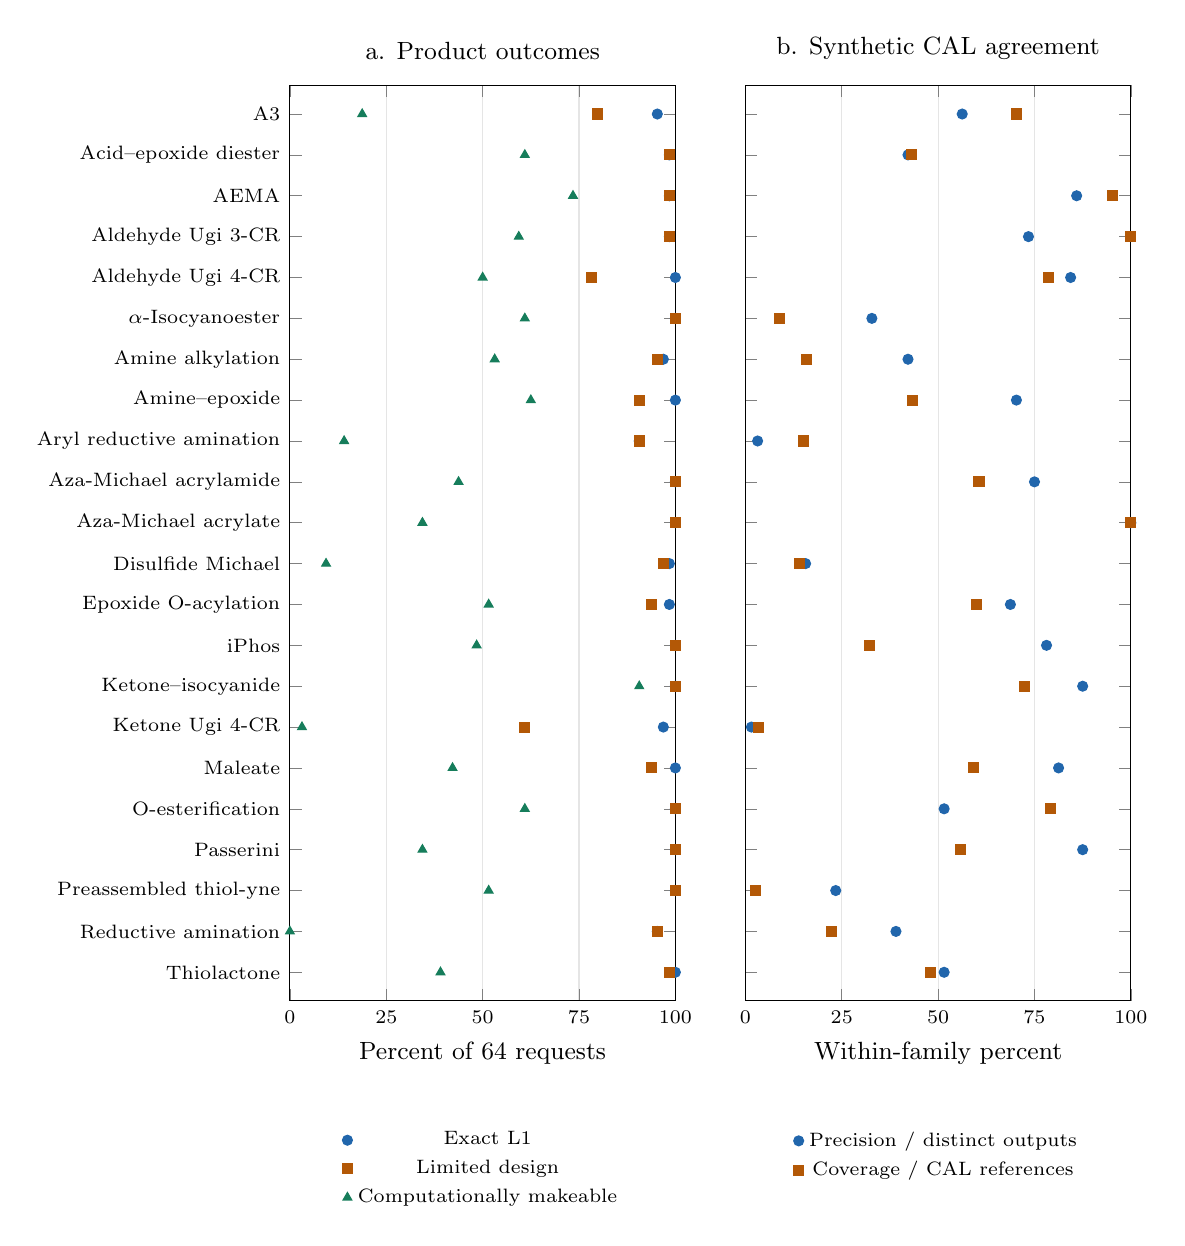
\begin{tikzpicture}
\begin{axis}[width=2.55in,height=5.2in,xmin=0,xmax=100,xtick={0,25,50,75,100},ymin=-.7,ymax=21.7,y dir=reverse,ytick={0,...,21},tick label style={font=\scriptsize},label style={font=\small},title style={font=\small},xmajorgrids=true,grid style={gray!20},legend style={font=\scriptsize,draw=none,at={(.5,-.13)},anchor=north},legend columns=1,name=left,yticklabels={{A3},{Acid--epoxide diester},{AEMA},{Aldehyde Ugi 3-CR},{Aldehyde Ugi 4-CR},{$\alpha$-Isocyanoester},{Amine alkylation},{Amine--epoxide},{Aryl reductive amination},{Aza-Michael acrylamide},{Aza-Michael acrylate},{Disulfide Michael},{Epoxide O-acylation},{iPhos},{Ketone--isocyanide},{Ketone Ugi 4-CR},{Maleate},{O-esterification},{Passerini},{Preassembled thiol-yne},{Reductive amination},{Thiolactone}},title={a. Product outcomes},xlabel={Percent of 64 requests}]
\addplot[only marks,mark=*,mark size=1.8pt,color=forgeblue] coordinates {(95.312500,0) (98.437500,1) (98.437500,2) (98.437500,3) (100.000000,4) (100.000000,5) (96.875000,6) (100.000000,7) (90.625000,8) (100.000000,9) (100.000000,10) (98.437500,11) (98.437500,12) (100.000000,13) (100.000000,14) (96.875000,15) (100.000000,16) (100.000000,17) (100.000000,18) (100.000000,19) (95.312500,20) (100.000000,21)};
\addlegendentry{Exact L1}
\addplot[only marks,mark=square*,mark size=1.8pt,color=forgeorange] coordinates {(79.687500,0) (98.437500,1) (98.437500,2) (98.437500,3) (78.125000,4) (100.000000,5) (95.312500,6) (90.625000,7) (90.625000,8) (100.000000,9) (100.000000,10) (96.875000,11) (93.750000,12) (100.000000,13) (100.000000,14) (60.937500,15) (93.750000,16) (100.000000,17) (100.000000,18) (100.000000,19) (95.312500,20) (98.437500,21)};
\addlegendentry{Limited design}
\addplot[only marks,mark=triangle*,mark size=1.8pt,color=forgegreen] coordinates {(18.750000,0) (60.937500,1) (73.437500,2) (59.375000,3) (50.000000,4) (60.937500,5) (53.125000,6) (62.500000,7) (14.062500,8) (43.750000,9) (34.375000,10) (9.375000,11) (51.562500,12) (48.437500,13) (90.625000,14) (3.125000,15) (42.187500,16) (60.937500,17) (34.375000,18) (51.562500,19) (0.000000,20) (39.062500,21)};
\addlegendentry{Computationally makeable}
\end{axis}
\begin{axis}[width=2.55in,height=5.2in,xmin=0,xmax=100,xtick={0,25,50,75,100},ymin=-.7,ymax=21.7,y dir=reverse,ytick={0,...,21},tick label style={font=\scriptsize},label style={font=\small},title style={font=\small},xmajorgrids=true,grid style={gray!20},legend style={font=\scriptsize,draw=none,at={(.5,-.13)},anchor=north},legend columns=1,at={(left.east)},anchor=west,xshift=.35in,yticklabels=\empty,title={b. Synthetic CAL agreement},xlabel={Within-family percent}]
\addplot[only marks,mark=*,mark size=1.8pt,color=forgeblue] coordinates {(56.250000,0) (42.187500,1) (85.937500,2) (73.437500,3) (84.375000,4) (32.812500,5) (42.187500,6) (70.312500,7) (3.174603,8) (75.000000,9) (100.000000,10) (15.625000,11) (68.750000,12) (78.125000,13) (87.500000,14) (1.562500,15) (81.250000,16) (51.562500,17) (87.500000,18) (23.437500,19) (39.062500,20) (51.562500,21)};
\addlegendentry{Precision / distinct outputs}
\addplot[only marks,mark=square*,mark size=1.8pt,color=forgeorange] coordinates {(70.370370,0) (43.157895,1) (95.238095,2) (100.000000,3) (78.688525,4) (8.737864,5) (15.789474,6) (43.243243,7) (15.189873,8) (60.606061,9) (100.000000,10) (14.062500,11) (60.000000,12) (32.258065,13) (72.413793,14) (3.448276,15) (59.183673,16) (79.069767,17) (55.882353,18) (2.638522,19) (22.222222,20) (47.916667,21)};
\addlegendentry{Coverage / CAL references}
\end{axis}
\end{tikzpicture}
\end{document}
